\chapter{Modello teorico di Controllo}\label{cap:controlModel}

\begin{minipage}{12cm}\textit{Se lo si desidera, utilizzare questo spazio per inserire un breve riassunto di ci\`o che verr\`a detto in questo capitolo. Inserire solo i punti salienti.}
\end{minipage}

\vspace*{1cm}

\section{Obiettivo di controllo}
Come accennato nella sezione "\nameref{sub:parametriMisurati}", attraverso il controllo e attuazione della corrente nel Primario del trasformatore, si punta controllare la corrente presente sul primario del trasformatore, e sempre come detto nella sezione "\nameref{sub:parametriMisurati}", non essendo possibile misurare la corrente di plasma direttamente, si usa la sua misura indiretta che passa per la $ F_{em} $.\\
In questa tesi l'obiettivo che ci si è ripromessi di raggiungere è la creazione di un controllo ad errore nullo sulla corrente di plasma.\vspace{-4mm}
\begin{figure}[h]
	\centering
	\caption[Sistema da controllare a blocchi con $ P(s) $]{Sistema da controllare a blocchi con $ P(s) $}
	\vspace{1mm}
	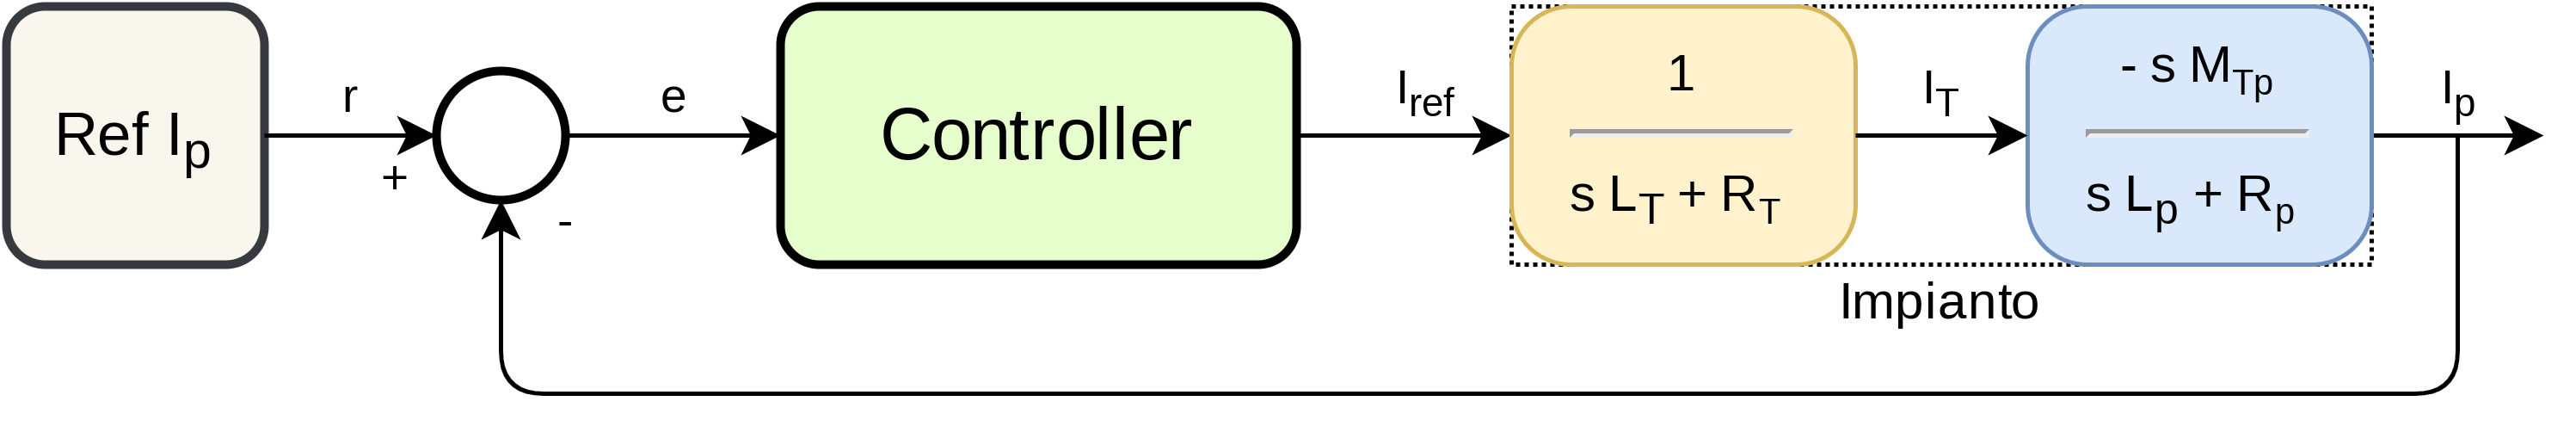
\includegraphics[width=1\textwidth]{ModelloMatematico/SchemiBlocchi.png}
\end{figure}\vspace{-4mm}

\noindent
Come visto però nella sezione, "\nameref{sub:parametriMisurati}", la misura a nostra disposizione il voltmetro la $V_2$, che equivale alla  diagnostica di $ V_{loop} $ in un impianto reale.\\
Dall'equazione della dinamica del plasma \ref{eq:correntePlasmaDinamica} siamo in grado di ricavare che:
\begin{empheq}[box=\mathStep]{equation*}
	V_2 = I_p \cdot R_p = F_{em} - L_p \cdot \dot{I_p}
\end{empheq}

\noindent
La quale, trascurando la dinamica del filtro RC di misura (che comunque è $ >= f_{tic} $ di acquisizione e di conseguenza ha una dinamica estremamente più rapida del segnale da misurare)  permette di ricavare, invertendo il segno della tensione come della corrente per avere i segni positivi, la funzione di ingresso-uscita dalla $ I_{ref} $ alla $ V_2 $ pari a:
\begin{empheq}[box=\mathCalc]{equation}
	V_2(s) = I_p(s) \cdot- R_p \Rightarrow V_2(s) = P_{pos}(s) \cdot I_{ref}(s) \cdot R_p
\end{empheq}
Da cui la funzione di trasferimento complessiva diventa:
\begin{empheq}[box=\mathCalc]{equation}\label{eq:FunxTrasImpiantoIrefV2}
	\frac{V_2(s)}{I_{ref}(s)} = P_{pos}(s) \cdot R_p
\end{empheq}
E il riferimento di corrente di plasma, diventa un riferimento di tensione secondo l'equazione di conversione:
\begin{empheq}[box=\mathCalc]{equation}\label{eq:V2RefEquivalent}
	V_{2_{ref}} = I_{p_{ref}} \cdot R_p
\end{empheq}

\begin{figure}[h]
	\centering
	\caption[Sistema da controllare ingresso-uscita reale]{Sistema da controllare ingresso-uscita reale}
	\vspace{1mm}
	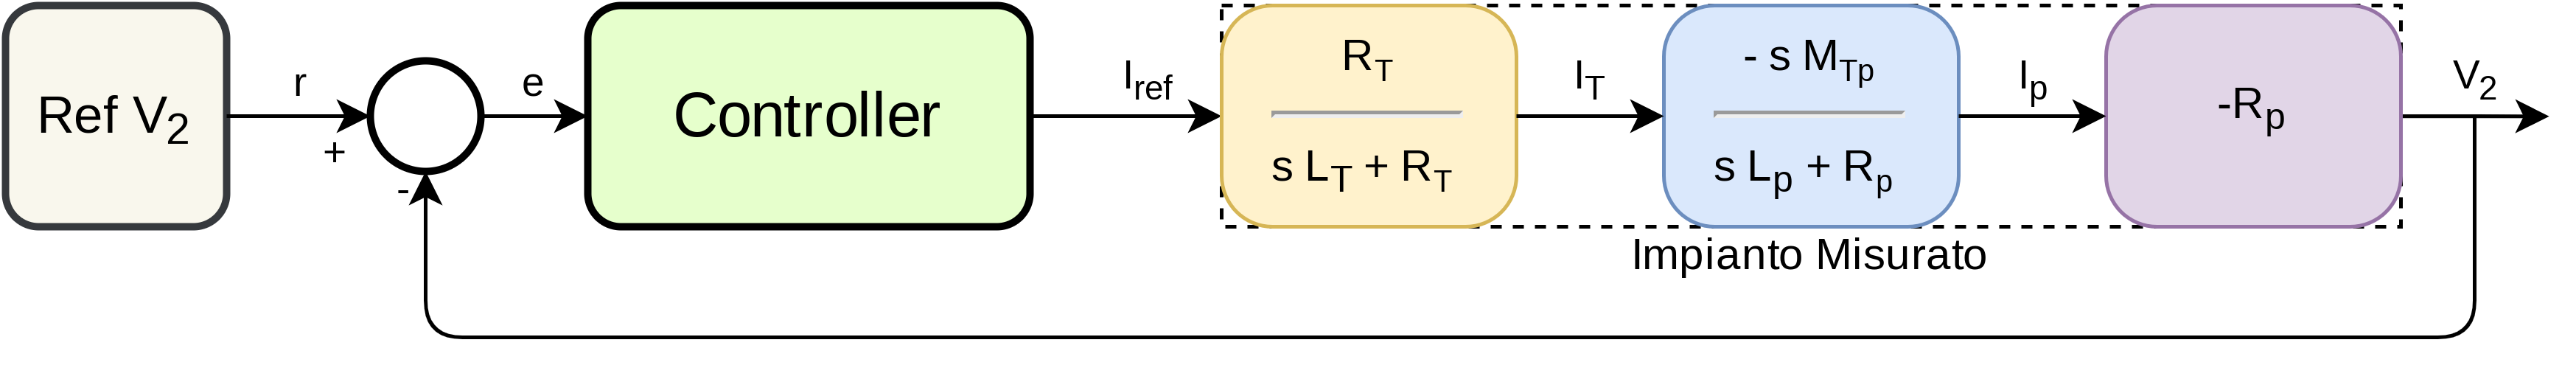
\includegraphics[width=1\textwidth]{ModelloMatematico/SchemiBlocchi-SchemaBlocchiV2Out.png}
\end{figure}

\newpage
\section{Teorema del valore iniziale e del valore finale}
Prima di procedere con il calcolo del controllore per i nostri scopi, è bene ricordare il \nameref{th:valIniziale} e il \nameref{th:valFinale} della Trasformata di Laplace (\cite*{Laplace}):

\begin{teorema}[Teorema del valore iniziale \label{th:valIniziale}]
	Se una funzione reale $ f  $ ha trasformata razionale $ F(s) $ con grado del denominatore maggiore del grado del numeratore (vale comunque sotto ipotesi ancora più larghe , purché $ F $ sia non razionale e $ f(0^+) $ esista) allora:
	\begin{empheq}[box=\mathResult]{equation} \label{eq:valIniziale}
		f(0^+) = \lim\limits_{s \rightarrowtail \infty} s \cdot F(s)
	\end{empheq}
\end{teorema}

\begin{teorema}[Teorema del valore finale \label{th:valFinale}]
	Se una funzione reale $ f  $ ha trasformata razionale $ F(s) $ con grado del denominatore maggiore del grado del numeratore e \underline{radici del denominatore (\textbf{poli}) nell’origine e o a parte reale negativa},\\
	allora:
	\begin{empheq}[box=\mathResult]{equation} \label{eq:valIniziale}
		\lim\limits_{t \rightarrowtail \infty} f(t) = \lim\limits_{s \rightarrowtail 0} s \cdot F(s)
	\end{empheq}
\end{teorema}

Questi 2 Teoremi chiave, permettono di risolvere comodamente le equazioni differenziali, e quindi calcolare in maniera semplice il controllore che permette di ottenere gli obiettivi di controllo che ci si è prefissati di ottenere.

\newpage

\section{Controllo a errore nullo} \label{sec:inseguitoreErroreNullo}
Definiamo ora $ P_m(s) $ come l'impianto Reale misurato tra la corrente di riferimento $ I_{ref} $ del primario, e la tensione del campo elettrico $ V_2 $ sul secondario.\\
Ne segue che la funzione di trasferimento complessiva è pari a:
\begin{empheq}[box=\mathCalc]{equation}\label{eq:impiantoMisurato}
	P_m(s)= \frac{V_2(s)}{I_{ref}(s)} = \frac{s M_{Tp} \cdot R_p}{( s L_p + R_p)(s L_T + R_T)} = \frac{s M_{Tp} \cdot R_p}{s^ 2L_p L_T + s(L_p R_T + L_T R_p) + R_p R_T}
\end{empheq}
Essendo il nostro obiettivo quello di portare $ e \rightarrowtail 0$ per $ t\rightarrowtail \infty $ con riferimenti $ r = cost $, ci calcoliamo la funzione sensitività $ W_{er}(s) $ (\textit{sensitivity transfer function}) e con il \nameref{th:valFinale} progetteremo il controllore $ C(s) $ che realizza l'obiettivo:\\
\begin{vwcol}[widths={0.5,0.5}, sep=8mm, rule=0px]
	\vspace{-12mm}
	\begin{empheq}[box=\mathStep]{equation*}
		W_{er}(s) = \frac{e(s)}{r(s)} = \frac{1}{1 + P_m(s)C(s)}
	\end{empheq}
	\newpage
	{\color{red} Sensitivity transfer function}
\end{vwcol}
\vspace{5mm}
\begin{vwcol}[widths={0.5,0.5}, sep=8mm, rule=0px]
	\vspace{-8mm}
	\begin{empheq}[box=\mathStep]{equation*}
		r(t) = cost \rightarrow r(s)= \frac{K_r}{s}
	\end{empheq}
	\newpage
	Trasformata di Laplace del riferimento
\end{vwcol}

Da cui, applicando il \nameref{th:valFinale} otteniamo:
\begin{empheq}[box=\mathCalc]{equation} \label{eq:dinamicaErroreRifCostFunxTrasf}
	\lim\limits_{t \rightarrowtail \infty} e(t) = \lim\limits_{s \rightarrowtail 0} s \cdot W_{er}(s) \cdot r(s) = s \cdot \frac{K_r / s}{1 + P_m(s)C(s)}
\end{empheq}

\begin{oss} \label{oss:Fattorizzazione}
	Al fine di semplificare il design del controllore, fattorizziamo ora $ P_m(s) $ e $ C(s) $ nella seguente forma, tralasciando così i dettagli dei termini non utili ai fini del design del controllore.
	\begin{vwcol}[widths={0.45,0.55}, sep=8mm, rule=0px]
		\vspace{-6mm}
		\begin{empheq}[box=\mathStep]{equation*}
			C(s) = K_c \cdot \frac{s^{\rho_{c_n}} \cdot C_n}{s^{\rho_{c_d}} \cdot C_d} = 
			\frac{K_c}{s^{\rho_{c}}} \cdot \frac{C_n}{C_d}
		\end{empheq}
		\newpage
		\begin{spacing}{1.25}
			{\footnotesize
				\begin{itemize}[itemsep=-1mm]
					\item $ K_c $ Guadagno statico Controllore.
					\item $ C_n $ Polinomio numeratore \underline{senza Zeri in 0}.
					\item $ C_d $ Polinomio denominatore \underline{senza Poli 0}.
					\item $ \rho_c $ è il grado del polo in 0 ($ \rho_{c_d} - \rho_{c_n} $).
				\end{itemize}
			}
		\end{spacing}
	\end{vwcol}
	
	\noindent\rule[0.5ex]{\linewidth}{0.5pt}
	
	\begin{vwcol}[widths={0.45,0.55}, sep=8mm, rule=0px]
		\vspace{-6mm}
		\begin{empheq}[box=\mathStep]{equation*}
			P_m(s) = K_p \cdot \frac{s^{\rho_{p_n}} \cdot P_n}{s^{\rho_{p_d}} \cdot P_d} = 
			\frac{K_p}{s^{\rho_{p}}} \cdot \frac{P_n}{P_d}
		\end{empheq}
		\newpage
		\begin{spacing}{1.25}
			{\footnotesize
				\begin{itemize}[itemsep=-1mm]
					\item $ K_c $ Guadagno statico Controllore.
					\item $ C_n $ Polinomio numeratore \underline{senza Zeri in 0}.
					\item $ C_d $ Polinomio denominatore \underline{senza Poli 0}.
					\item $ \rho_p $ è il grado del polo in 0 ($ \rho_{p_d} - \rho_{p_n} $).
				\end{itemize}
			}
		\end{spacing}
	\end{vwcol}
\end{oss}
\newpage
Partendo da questa forma, svolgiamo i calcoli dell'equazione  \ref{eq:dinamicaErroreRifCostFunxTrasf}:
\begin{empheq}[box=\mathCalc]{equation} \label{eq:guadagnoAnelloPlusOne}
	1 + P_m(s)C(s) =  1 + \frac{K_c}{s^{\rho_{c}}} \frac{C_n}{C_d}\cdot \frac{K_p}{s^{\rho_{p}}}  \frac{P_n}{P_d}=
	\frac{s^{\rho_{c} + \rho_{p}} C_d P_d + K_c K_p C_n P_n}{s^{\rho_{c} + \rho_{p}} C_d P_d}
\end{empheq}

Da cui otteniamo che:
\begin{center}
	{\large
		$ s \cdot W_{er}(s) \cdot r(s) =
			\cancel{s} \cdot \frac{K_r/\cancel{s}}{1 + P_m(s)C(s)} =
			K_r \cdot \left(\frac{s^{\rho_{c} + \rho_{p}} C_d P_d + K_c K_p C_n P_n}{s^{\rho_{c} + \rho_{p}} C_d P_d}\right)^{-1} \Rightarrow$
	}
\end{center}

\begin{empheq}[box=\mathStep]{equation*}
	\lim\limits_{t \rightarrowtail \infty} e(t) = \lim\limits_{s \rightarrowtail 0} s \cdot W_{er}(s) \cdot r(s) = \lim\limits_{s \rightarrowtail 0}
	K_r \cdot \frac{{\color{fireenginered}s^{\rho_{c} + \rho_{p}}} \cdot C_d P_d}{{\color{fireenginered}s^{\rho_{c} + \rho_{p}}} \cdot C_d P_d + K_c K_p C_n P_n}
\end{empheq}
Tenendo presente che $ C_d,P_d,C_n,P_n \rightarrowtail 1 $ per $ s \rightarrowtail 0 $, poiché gli Zeri sono stati fattorizzati fuori assieme al guadagno Statico (vedi osservazione \ref{oss:Fattorizzazione}), abbiamo che gli esiti per l'errore a \textit{Steady state}(Stato Stazionario) dipendono solo dal grado di {\color{fireenginered}$ \rho = \rho_{c} + \rho_{p} $ con $ \rho \in \mathbb{Z} $} e sono pari a:

\begin{center}	\label{eq:esitiErrore}
	$ e_\infty = \lim\limits_{t \rightarrowtail \infty} e(t) =
		\left \{ \begin{array}{l c c}
			0                   & se & \rho \geq 1  \\
			\frac{K_r}{K_c K_p} & se & \rho = 0     \\
			\infty              & se & \rho \leq 0 
		\end{array}
		\right.
	$
\end{center}
Essendo {\color{fireenginered}$ \rho_{p} = -1 $} a causa dello Zero in 0, abbiamo che il controllore dovrà necessariamente avere {\color{fireenginered}$ \rho_{c} = 2 $} per ottenere {\color{fireenginered}$ \rho = 1 $}. Il grado minimo di controllore di cui necessitiamo è quindi:
\begin{empheq}[box=\mathStep]{equation*}
	C(s) = \frac{1}{s^2}
\end{empheq}
Questo controllore base è complicabile a piacere aggiungendo altri Poli e Zeri stabili, con l'obiettivo di migliorarne le performance della risposta del sistema.
\begin{oss}
	Il controllore descritto in \ref{eq:controllerStructure}, anche se stabilizza il sistema e lo rende un \underline{inseguitore ad errore nullo}, \textbf{non è stabile}.\\
	Esso infatti ha 2 poli in 0, rendendolo un polo \underline{non semplice} e quindi causa di instabilità polinomiale.\\
	Questa conseguenza non è evitabile, ed è bene accetta poiché permette di inseguire con errore nullo, per la durata dell'esperimento, il riferimento.\\
	Bisognerà ovviamente tenerne conto in fase di realizzazione poiché con il procedere del tempo dell'esperimento, i numeri dello stato diventeranno sempre maggiori, e ciò potrà portare a problemi di overflow numerici.
\end{oss}

\newpage
\noindent
La dinamica $ e_\infty $ riportata (\ref{eq:esitiErrore}) è valida se il sistema a ciclo chiuso $ W_{V_2 r}(s) $ risulta Asintoticamente Stabile, analizziamo quindi la sua stabilità:\\
\begin{vwcol}[widths={8cm,8cm}, sep=0mm, rule=1px]
	\vspace{-7.15mm}
	\begin{empheq}[box=\mathStep]{equation*}
		W_{V_2 r}(s) = \frac{V_2(s)}{r(s)} = \frac{P_m(s)C(s)}{1 + P_m(s)C(s)}
	\end{empheq}
	\newpage
	{\color{red} Complementary Sensitivity \\ Transfer Function}
\end{vwcol}
\noindent
E la stabilità di questa funzione è data dai poli del suo denominatore, che abbiamo già calcolato \ref{eq:guadagnoAnelloPlusOne}, e la cui formula è:

\begin{center}
	{\large $ Den(W_{V_2 r}) = {\color{fireenginered}s^{\rho_{c} + \rho_{p}}} C_d P_d = {\color{fireenginered}s^{\rho}} C_d P_d$} \hspace{8mm} ($ C_d $ e $ P_d $ senza poli nell'origine \footnote{Nota Bene: $ P_d $ e $ C_d $ sono il risultato della fattorizzazione vista sopra nell'osservazione \ref{oss:Fattorizzazione}, non possono quindi esserci poli nell'origine in questi 2 termini \textbf{per costruzione}})
\end{center}
Partendo dalla conoscenza che $ P_d $ è sicuramente composta da poli stabili nel semipiano $ \mathbb{C^-} $ (vedi sezione \nameref{TrasformatoreModelloTokamak}), da cui segue che qualunque polo stabile per il controllore ($ C_d $) non destabilizza il sistema e rende valida la dinamica $ e_\infty $ riportata prima (\ref{eq:esitiErrore}), e anzi, il numeratore del controllore può tranquillamente essere instabile, se dovesse servire.

\subsection{Design di controllore adottato}
In questa tesi la forma di controllore che si è scelto di usare è la seguente:
\begin{empheq}[box=\mathCalc]{equation} \label{eq:controllerDesign}
	C(s) = \frac{K_2}{s^2} + \frac{K_1}{s} + K_p = \frac{K_2 + s K_1 + s^2 K_p}{s^2}
\end{empheq}
\noindent
La scelta è dovuta alla sua somiglianza con un più classico PID, che in questo caso non sarebbe bastato a raggiungere le specifiche (vedi sezione \nameref{sec:inseguitoreErroreNullo}), ma come per lui, tramite un lavoro di \textit{Tuning} dei coefficienti è possibile ottenere delle buone prestazioni per il sistema a ciclo chiuso.\\
Ulteriore vantaggio di questa struttura è che permettere un semplice controllo switching, variando i coefficienti del numeratore, in base alla fase dell'esperimento.

\newpage

\section{Simulazione \textit{Qualitativa} su Simulink}
Partendo dal modello stimato che si è ottenuto nel capitolo "\nameref{cap:stimaModello}" in cui si è giunti al modello nell'equazione \ref{eq:StimaModelloInOut}, puntiamo ora a testare il controllo base che abbiamo teorizzato e successivamente la sua evoluzione "\textit{PID-style}"














